\chapter{zamk Integration Framework}
\chapterprecis{In this chapter we introduce a light-weight component integration framework, which is based on composable integration modules.}

%\epigraph{text}{source}

\section{Introduction}
Systems are often faced with new requirements for adding new functionality or updating what is already there. 
A preferred way of extending or updating system behavior is through adding components. 
A software component can be described as a self-contained entity with a well-defined interface and behavior. 
Components can be plugged into target systems to extend the system with their provided functionality.
The target system contains data about the state of the system which is required by the component. 
In order to establish the data flow, connections should be made between the system and the component; this operation is usually referred as component integration or component binding. 

Depending on the extensibility of the software architecture this task can be very difficult. 
In large software systems, traditional middleware approaches such as CORBA, DCOM or JRMI can be used to manage the complexity introduced by inter-component dependencies. 
These middleware solutions are geared towards providing built-in support for widely-used technologies and offer little support for customization. 
For smaller systems, using such software can be inefficient, since they are intended to be used for component integration in enterprise software and their adoption is itself complex and requires effort. Therefore, for such systems component integration is manually implemented. Component integration is trivial when the target system and the component have a common interface. However in most cases the integration introduces the requirement that the interfaces should be made compatible with each other to make the final system functional.

This is a known problem and its solution is captured in the \emph{adapter pattern} (cite Gamma). 
Typically adapters are tailored for a given integration. 
The complexity of the adapters depend on the complexity of the structures they adapt from and to. 
For a simple type conversion between classes with small number of fields that have primitive types, the adapter is not very complex and it can be easily maintained when either of the classes change. 
However for classes which contain fields of other types, which themselves are composite, the adapter implementation becomes more complex.
This results in adapter implementations that hide the \emph{ugly} adaptation code, which are fragile against software evolution and which are not reusable. 

Another common observation is that the adapters are hard to come by in their true form, i.e. their definition as a design pattern. Usually ``adapters'' are used for assembling multiple objects or enriching the adaptee data by taking extra parameters. This additional functionality makes adapters more complex and less reusable. \TODO{Lack of Cohesion analysis of such adapters} 

Another important aspect of component integration is instance-level dependencies. 
Hence the other step of integration is assigning the data values to the relevant fields.  
Keeping the system and the components loosely coupled is an important principle of component-based design. 
Dependency injection (DI) (cite fowler) is a lightweight method for keeping modules loosely coupled by delegating the creation of concrete objects to so-called \emph{injectors}. This approach allows a customizable and a decoupled way of creating dependencies, while maintaining loose coupling.

In this chapter we introduce our component integration framework, Zamk, which unites dependency injection with \emph{under-the-hood} adaptation logic. The Zamk framework creates a registry of user-defined integration modules, which are composable entities. Zamk framework also comes with a concise domain-specific language called \textsf{gluer} to define dependency injections. Given a dependency injection statement the framework tries to build the \emph{type path} between the injectee and the injection field. We automate the adaptation process by exploiting the type hierarchies and provide checks and context-relevant messages for correct integration. The details of the framework will explained throughout the chapter.
 
\section{Motivation and Goals}

The goal of component integration is to make two components work together to provide a required functionality. However component integration efforts can be difficult to estimate, since the design and implementation of components vary greatly. Component models try to remedy this situation by defining the term component as ``\ldots a software element that conforms to a component model and can be independently deployed and composed without modification according to a composition standard.~\cite{Heineman2001}'' Unfortunately component models do not guarantee well-structured binding, since one cannot guarantee that every used component conforms to a single component model. The incompatibility starts on the model level which translates to the interface level. 

The code that binds components together is referred to as \emph{glue code}. This is an umbrella term which refers to all code that facilitate the ``hooking'' the components together and establish channels for information exchange. The overall effort spent on the glue code varies and is dependent on many other factors. In \cite{abts2000cocots}, the preliminary findings of a software integration life-cycle cost model for commercial-off-the-shelf (COTS) components is presented. It is stated that ``\ldots the the greatest COTS integration effort tends to be concentrated on glue code development''. Typically glue code is viewed as a one-time task during integration, which results in non-reusable implementation (\TODO{Problem Statement}).

\begin{figure}[h]
\centering
\inputtikz{0.90}{chapterzamk/images/components.tex}
%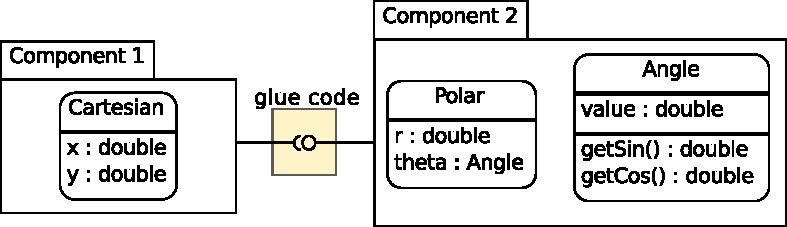
\includegraphics[width=0.7\textwidth]{chapterzamk/images/component.pdf}
\caption{Plugging a polar coordinate component to a cartesian component system}%
\label{fig:cartesian}%
\end{figure}

Let us illustrate our claim with a simple example. In Figure~\ref{fig:cartesian} two components are shown. \textsf{component1} contains one class called \textsf{Cartesian}. Now we would like to support also polar coordinates and \textsf{component2} provides this support. However all the existing data is in Cartesian coordinates and we need to convert in to polar coordinates. In order to make this conversion, one can write an adapter that looks like the one shown in Listing~\ref{lst:cart2polar}. The class \textsf{Cartesian2Polar} is an object adapter and it is a valid solution to the problem at hand. Note that \textsf{component2} also provides support for cylindrical and spherical coordinates, which are not used, thus not shown in the figure. 

\begin{lstlisting}[float, caption={A Cartesian to polar adapter}, label={lst:cart2polar}]
public class Cartesian2Polar extends Polar{
	Cartesian adaptee;
	public Cartesian2Polar(Cartesian c) {
		super();
		this.adaptee = c;
		super.setR(Math.sqrt(Math.pow(adaptee.getX(), 2) + Math.pow(adaptee.getY(), 2)));~\label{lst:cart2polar:setR}~
		super.setTheta(new Angle(Math.atan(adaptee.getY()/adaptee.getX())));~\label{lst:cart2polar:setTheta}~
	}
}
\end{lstlisting}

Now let's take a look at the situation where this system evolves. Now we would like to support three dimensional Cartesian coordinates. Therefore we extend the class \textsf{Cartesian} as \textsf{Cartesian3D}. This new feature gives us the opportunity to use the cylindrical and spherical coordinates provided by \textsf{component2}. Once again we need to write adapters to convert between \textsf{Cartesian3D} and \textsf{Spherical, Cylindrical} classes (\TODO{Figure evolved model}). 

\begin{lstlisting}[float, caption={Adapter for converting three dimensional cartesian coordinates to Cylindrical coordinates}, label={lst:cart3d2Cyn}]
public class Cart3D2Cylindrical extends Cylindrical {
	Cartesian3D adaptee;
	public Cart3D2Cylindrical(Cartesian3D adaptee) {
		super(0, null, 0);
		this.adaptee = adaptee;
		super.setR(Math.sqrt(Math.pow(adaptee.getX(), 2) + Math.pow(adaptee.getY(), 2))); ~\label{lst:cart3d:setR}~
		super.setTheta(new Angle(Math.atan(adaptee.getY()/adaptee.getX()))); ~\label{lst:cart3d:setTheta}~
		super.setZ(adaptee.getZ());
	}
}
\end{lstlisting}
\begin{lstlisting}[float, caption={Adapter for converting three dimensional cartesian coordinates to Spherical coordinates}, label={lst:cart3d2Sph}]
public class Cart3D2Spherical extends Spherical {
	Cartesian3D adaptee;
	public Cart3D2Spherical(Cartesian3D adaptee) {
		super(0, null, null);
		this.adaptee = adaptee;
		super.setRho(Math.sqrt(Math.pow(adaptee.getX(), 2) + Math.pow(adaptee.getY(), 2) + Math.pow(adaptee.getZ(), 2) )); ~\label{lst:cart3d:setRho}~
		super.setTheta(new Angle(Math.atan(adaptee.getY()/adaptee.getX()))); ~\label{lst:cart3d:setTheta2}~
		super.setPhi(new Angle(Math.atan(adaptee.getZ()/(Math.sqrt(Math.pow(adaptee.getX(), 2) +
				Math.pow(adaptee.getY(), 2))))));
	}
}
\end{lstlisting}

 
The implementation for \lstinln{Cartesian3D2Cylindrical} and \lstinln{Cartesian3D2Spherical} are shown in Listing~\ref{lst:cart3d2Cyn} and Listing~\ref{lst:cart3d2Sph} respectively. All of the adapters presented in these implementations have repeated lines of code. In Listing~\ref{lst:cart2polar} on line~\ref{lst:cart2polar:setR}, in Listing~\ref{lst:cart3d2Cyn} on line~\ref{lst:cart3d:setR} and in Listing~\ref{lst:cart3d2Sph} on line~\ref{lst:cart3d:setRho} all include the same calculation. In fact the calculations made in \lstinln{Cartesian2Polar} adapters appear in \lstinln{Cart3D2Cylindrical} and \lstinln{Cart3D2Spherical}. However the way \lstinln{Cartesian2Polar} is defined makes it impossible for us to reuse these calculations.\footnote{If Java supported multiple inheritance, we could have reused the \lstinln{Cartesian2Polar} adapter's code by declaring \lstinln{Cart3D2Cylindrical} as a subclass of both \lstinln{Cartesian2Polar} and \lstinln{Cylindrical}. However the lack of reuse would still be present in \lstinln{Cart3D2Spherical}.} 

\begin{lstlisting}[float, caption={Decomposition of the members of the polar coordinate}, label={lst:ctpdecomp}]
public class CartesianToAngleAdapter extends Angle{
	private Cartesian adaptee;
	public CartesianToAngleAdapter(Cartesian c)
	{
		super();
		this.adaptee = c;
		super.angle = Math.atan(adaptee.getY()/adaptee.getX());
	}	
}
public class Pythagoras{
	private Cartesian adaptee;
	public Pythagoras(Cartesian c)
	{
		this.adaptee = c;
		r = Math.sqrt(Math.pow(adaptee.getX(), 2) + Math.pow(adaptee.getY(), 2));
	}
	public double getAdaptedValue()
	{
		return r;
	}	
}
\end{lstlisting}

Let us re-design the adapter shown in Listing~\ref{lst:cart2polar}. Then we can have the decomposition shown in Listing~\ref{lst:ctpdecomp}. Using this decomposition we can create a \lstinln{Polar} object given a \lstinln{Cartesian} object \lstinln{c} by writing:
\begin{lstlisting}
Polar p = new Polar(new Angle(c), (new Pythagoras(c)).getAdaptedValue());
\end{lstlisting}

Furthermore we can reuse these classes to create a \lstinln{Cylindrical} object given a \lstinln{Cartesian3D} object \lstinln{c3d} as follows:
\begin{lstlisting}
Cylindrical cyn =  new Cylindrical(new Angle(c3d), (new Pythagoras(c3d)).getAdaptedValue(), c3d.getZ());
\end{lstlisting}

By decomposing the glue code into two reusable classes we were able to make the coordinate conversions in a modular manner. The classes we have defined so far are not sufficient for converting from \lstinln{Cartesian3D} to \lstinln{Spherical}. Still we can reuse these classes by extending them as seen on listing~\ref{lst:ctpdecomp2}.

\begin{lstlisting}[float, caption={Extended versions of conversion classes}, label={lst:ctpdecomp2}]
public class Cartesian3DToAngleAdapter extends CartesianToAngleAdapter{
	private Pythagoras pyth;
	public Cartesian3DToAngleAdapter(Cartesian3D c)
	{
		super(c);
		pyth = new Pythagoras(c);
		super.angle = Math.atan(adaptee.getZ()/pyth.getAdaptedValue());
	}	
}
public class Pythagoras3D extends Pythagoras{
	public Pythagoras3D(Cartesian3D c)
	{
		super(c);
		this.r = Math.sqrt(Math.pow(super.getAdaptedValue(), 2) + Math.pow(c.getZ(), 2));
	}	
}
\end{lstlisting}

Using the extended decomposition we can convert a \lstinln{Cartesian3D} object to a \lstinln{Spherical} object in the following manner.

 \begin{lstlisting}
Spherical sph =  new Spherical((new Pythagoras3D(c3d)).getAdaptedValue(),new CartesianToAngleAdapte(c3d), new Cartesian3DtoAngleAdapter(c3d))
\end{lstlisting}


Based on our observations on the reusability issues of glue code we have devised our goal to solve these issues. Our main idea is that given \emph{atomic adaptations}, it is possible to build a path between two types automatically using static analysis techniques and generate the glue code that binds these types together. Our focus is on the structural binding, which entails forming the static dependencies between components. In its most basic form this corresponds to injecting values to certain fields. At this level the requirement is to establish the type compatibility. This is achieved by obtaining the correct type that is injectable to a field by wrapping the injected value. 

Another issue we want to tackle is \emph{overloaded adapters}. Above we mentioned atomic adapters, by this we mean an adapter is a unit that only performs adaptation and nothing else. Therefore adapters are not sufficient to realize our goal, we need to have additional composition structures which assemble, enrich or compartmentalize these adapters. 

\TODO{Requirements}

\section{Background}
In this section we will give some background on the concepts that will be used as a part of our solution. 

\subsection{Adapter Pattern}
Adapter pattern is a design pattern that is used to translate an interface to a compatible interface. Adapters, also known as wrappers, can be implemented in two ways: as a \emph{class adapter} (Figure~\ref{fig:classadapter}), which uses multiple inheritance to adapt one interface to the other \emph{or} as an \emph{object adapter} (Figure~\ref{fig:objectadapter}), which uses object composition to adapt wrapped object to a specific interface. 

\begin{figure}[h]
\centering
\subfloat[The class adapter pattern]{\inputtikz{0.80}{chapterzamk/images/classadapter}
\label{fig:classadapter}%
}
\hfill
\subfloat[The object adapter pattern]{\inputtikz{0.80}{chapterzamk/images/objectadapter.tex}
\label{fig:objectadapter}%
}
\caption{Different versions of the adapter pattern}
\end{figure}




\section{Approach}

Our approach is an integration framework that marries dependency injection pattern with object adapters. In Figure~\ref{fig:main} an overview of the \zamk integration framework is shown. The framework consists of several components that work together and introduces a concise domain-specific language (DSL) called \gluer. \gluer~ is used to define dependencies between objects. The specifications written in \gluer~ is parsed by the \emph{Gluer parser}. 

\zamk uses a repository of composable \emph{integration modules} which are defined by the user. Integration modules can be adapters, enrichers, assemblers or splitters. The details of these modules will be explained in section~\ref{sec:zamk:modules}. When the user defines an injection between incompatible types, \emph{integration logic} component retrieves and assembles integration modules to convert the type of the injectee object to a compatible type expected by the injected field.

Finally the \emph{dependency injection component} performs the injection; this component supports two types of injection, constructor injection and setter injection. The details of this operation will be elaborated in section~\ref{sec:zamk:di}.

\begin{figure}
\centering
\def\svgwidth{\columnwidth}
%\input{chapterzamk/images/zamkoverview.pdf_tex}
 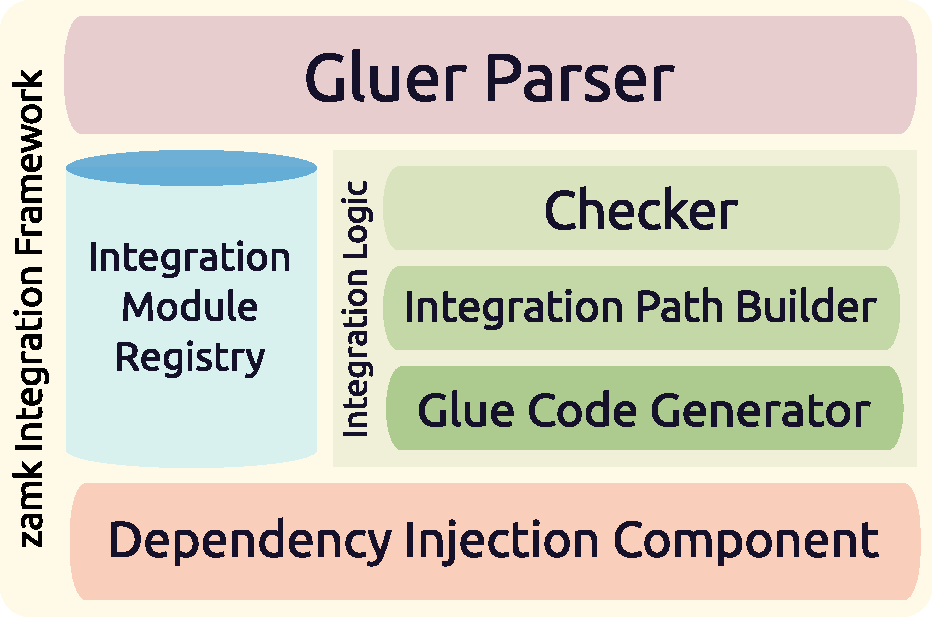
\includegraphics[width=0.75\textwidth]{chapterzamk/images/zamkoverview2.pdf}
\caption{An abstract view of the \zamk integration framework}
\label{fig:main}
\end{figure}

\subsection{The Gluer Language}
The \gluer~ language is a concise DSL that is designed to declare dependencies between fields and objects. Essentially the \gluer~ language is an external dependency injection declaration which triggers an internal logic that processes the injectee object. Therefore the \gluer~ language is not a plain dependency injection language. This is why we chose the keyword \lstinln{glue} instead of \lstinln{inject}. A simple gluer statement looks like the following:

\lstinline~glue <injection-field> with <injectee-object>~

\begin{description}
\item[<injection-field>] The injection field is a fully qualified name of a non-static field of a class. It can refer to any type, including primitive types. 
\end{description}

\begin{description}
\item[<injectee-object>] The injectee object represents the object to be processed and injected to the injection field. There are several options for creating this objects.
	\begin{description}
	\item[new] The \lstinline{new} statement is followed by a fully classified name of a class. This means, whenever an object is to be injected, it should be newly created using the \emph{default constructor} of the given class. 

	\item[single] Similar to \lstinline{new}, \lstinline{single} statement is followed by a fully qualified name of a class, which is instantiated when an injection is triggered. The difference is instead of creating a new object each time, a \emph{single} object is reused among injections.
	\TODO{possible use case}

	\item[retval] Short for ``return value'', this keyword is followed by a fully qualified reference to a method, which returns the object we would like to inject. When an injection is triggered, the method is called and the returned value is glued to the injection field.
	\end{description}
\end{description}

The \gluer~language also supports 1--to--many and many--to--1 gluing operations. \TODO{Expand}




\subsection{Integration Logic}
\label{sec:zamk:logic}
The integration logic is responsible for wrapping the what objects with appropriate adapters to be injected to where field. 
The what objects may need to be preprocessed before adaptation, a what object can be split into different objects (one-to-many) or multiple what objects can be assembled to a single object. 
These operations are done automatically by the integration logic. Figure~\textbf{ref} shows the flowchart of operations that take place for finding enrichers and assemblers for objects.

\TODO{flowcharts for integration modules}

\subsection{Integration Modules}
\label{sec:zamk:modules}
Integration modules are annotated intefaces which are registered by the \zamk run-time. The annotations include information about the type of the module and how the generated implementation of that modules should behave. The integration logic composes these modules to obtain the correct type-conversion. The details of the different integration modules offered by the \zamk framework is explained below.


\subsubsection{Adapters}
\zamk adapters are object adapters (Figure~\ref{fig:objectadapter}) and are implemented as plain Java classes that are annotated with the \lstinln{@Adapter} keyword. 
In order to identify the target and the adaptee types, we rely on the declarations of the adapter class.
We assume target type is the declared super-type of the adapter. 
If no super-type is declared, then we assume \lstinln{java.lang.Object} is the super-type.
The adaptee type is inferred from the type of the argument that is required by the single paramter constructor of the Adapter class. 
With this inference mechanism we also enforce constraints to the adapter definition.
First, the target super-type can only be a class and by using Java's single inheritance property we can ensure that there's only one such super-type. 
Second, we limit the number of single argument constructors of the adapter classes to one, to avoid ambiguity.

We have opted for having these constraints instead of embedding the adapter meta-information into the annotation, we think that having these constraints will yield \emph{pure} adapters which represent one-to-one conversions between types. 

When the adapters defined in Listing~\ref{lst:ctpdecomp} are annotated with \lstinln{@Adapter}, by looking at the extended types and the single argument constructors they will be registered as follows (\lstinln{adapter name -> (adaptee, target)}): \lstinln{CartesianToAngleAdapter -> (Cartesian, Angle)} and \lstinln{Pythagoras -> (Cartesian, int)}. 

Note that the adapter \lstinln{Pythagoras} represents a special case where the target type is a primitive type.
Since wrapper classes of primitive types are \lstinln{final} they cannot be extended.
To handle this limitation (and the case of final classes), the user can implement the \lstinln{getAdaptedValue()} method, which is recognized by \zamk, to obtain the resulting adapted value. 
The limitation of this strategy is that an instance of the \lstinln{Pythagoras} class cannot be directly used as a parameter instead of an \lstinln{Integer} type. 





\subsubsection{Assemblers}
Assemblers are Java interfaces that are annotated with \lstinln{@Assembler} keyword. 
The \lstinln{@Assembler} annotation enforces that the interface declares at least a method called \lstinln{assemble}, which returns a \emph{non-primitive} type. 
The return type of the \lstinln{assemble} method specifies which type the assembler produces and is also registered.
The \lstinln{@Assembler} annotation requires a \lstinln{type} argument to specify what type of object creation medium it will utilize. 
Currently we support two types; constructor and factory. 
In Listing~\ref{lst:assembler1} an assembler called \lstinln{PolarAssembler} is declared. 

When the constructor is used for assembly, we check if the return type of the \lstinln{assemble} method is an interface. 
Since interfaces cannot declare constructors, we emmit a compile error indicating that interfaces are not acceptable with this type of assembly. 
\begin{lstlisting}[float, caption={An example Assembler with ``constructor'' type}, label={lst:assembler1}]
@Assembler("constructor")
public interface PolarAssembler{
	public component2.Polar assemble(double r, Angle the);
}
\end{lstlisting}
If the return type, in this case \lstinln{Polar}, is a class then we search for the constructors which accept the same arguments with the same lexical order as in the \lstinln{assemble} method.
\TODO{Note that \lstinln{assemble} method can be overloaded.}
In the absence of such a constructor a compile error is emmited to notify the user. 
When the constructor is found, the impementation class is generated during compile time.  
The generated implementation for the \lstinln{PolarAssembler}~(Listing~\ref{lst:assembler1}) is shown in Listing~\ref{lst:assembler1impl}.
\begin{lstlisting}[float, caption={The generated implmentation of the \lstinln{PolarAssembler} in Listing~\ref{lst:assembler1}}, label={lst:assembler1impl}]
public class PolarAssemblerImpl implements PolarAssembler {
	public component2.Polar assemble(double r, component2.Angle the) {
		return new component2.Polar(r, the);
	}
}
\end{lstlisting}

\TODO{Factory}

\subsubsection{Splitters}
\begin{enumerate}
\item how are they defined; regular classes with @Splitter annotation, They should implement the ISplitter interface which comes with the split(Object) method
\item How are they registered, we may need some meta information
\end{enumerate}



\textbf{The flowchart from Arnout about adapter retrieval}

\subsubsection{Adapter Resolution}
Precedence rules

Informative error messages
\subsection{Dependency Injection}\label{sec:zamk:di}

\section{Module Retrieval Algorithm}
\section{Checks}
\section{Evaluation}
\section{Integration of instance pointcuts with Integration framework}
